%
% teil3.tex -- Beispiel-File für Teil 3
%
% (c) 2020 Prof Dr Andreas Müller, Hochschule Rapperswil
%
% !TEX root = ../../buch.tex
% !TEX encoding = UTF-8
%
\section{Anwendung des genetische Algorithmus
\label{variationsprinzip_algorithmen:section:genetic_algorithm_process}}
\rhead{Teil 3}
Der Genetische Algorithmus nutzt nach ChatGPT das Variationsprinzip 
und dies wird mit nachfolgender Aussage so definiert.
\\
\\
Das Variationsprinzip ist ein grundlegendes Konzept in der 
evolutionären Computertechnik, insbesondere in genetischen 
Algorithmen. Es besagt, dass genetische Vielfalt in einer 
Population von Individuen aufrechterhalten werden muss, 
um eine effektive Suche im Suchraum zu ermöglichen und eine 
Lösung für das zugrunde liegende Problem zu finden.
\\
Der genetische Algorithmus nutzt dieses Variationsprinzip, um eine 
Population von möglichen Lösungen zu einem Problem zu entwickeln 
und zu verfeinern.\cite{chatgpt2024}

In den nächsten Abschnitt wird der Ablauf des genetischen Algorithmus 
auf das Travelling Salesman Problem angepasst und angeschaut, das Kapitel
konzentiert sich eher auf den logischen Ablauf und weniger, um die 
Mathematischen Berechnung.

%
% teil3.tex -- Beispiel-File für Teil 3
%
% (c) 2020 Prof Dr Andreas Müller, Hochschule Rapperswil
%
% !TEX root = ../../buch.tex
% !TEX encoding = UTF-8
%
\subsection{Initialisierung
\label{genetic_algorithm:initialization}}
\rhead{Initialisierung}
Der Startpunkt des genetischen Algorithmus ist die Initialisierung.
Dabei wird eine zufällige Population von möglichen Lösungen erstellt.
Diese wird als ein genetischer String dargestellt.

\begin{figure} [h]
	\centering
	
\includegraphics[width=0.8\textwidth]{
        papers/variationsprinzip_algorithmen/images/teil3/01_genetic_string.png
        }
	\caption{Beispiel eines möglichen genetischen Strings}
	\label{fig:possible_genetic_string}
\end{figure}

In jeder Position kann ein Gen aktiviert (1) oder deaktiviert (0) sein.
Diese Darstellung eignet sich jedoch nicht für das Travelling Salesman 
Problem (TSP), da eine Stadt nicht einfach ein- oder ausgeschaltet werden kann.
Auf die Wege ist es auch nicht anwendbar, das dann immer nur 1 Weg der vielen Wege 
aktiviert werden kann. Im TSP ist die Reihenfolge der Städte entscheidend. 
Daher wird die jeweilige Nummer der Stadt verwendet, wie im folgenden Bild 
\cite{cities_genetic_string} dargestellt:

\begin{figure} [h]
	\centering
	\includegraphics[width=0.8\textwidth]{
        papers/variationsprinzip_algorithmen/images/teil3/02_genetic_string_cities.png
        }
	\caption{Beispiel von Städten in einem genetischen String dargestellt}
	\label{fig:cities_genetic_string}
\end{figure}

Anstatt alle möglichen Lösungen zu erstellen, wird nur ein kleiner Teil 
(Population) zufällig generiert und weiter bearbeitet. Diese Taktik 
spart Zeit und Ressourcen.

Die zufällige Erzeugung der Anfangspopulation stellt ebenfalls eine Form 
der Variation dar. Sie sorgt dafür, dass die Suche nicht von einem begrenzten 
Bereich des Lösungsraums startet, sondern eine breite Palette von möglichen 
Lösungen berücksichtigt. Dabei werden jedoch keine Berechnungen durchgeführt, 
sondern zufällige Lösungen erstellt, in der Hoffnung, dass eine davon nahe 
an das Optimum herankommt.


%
% teil3.tex -- Beispiel-File für Teil 3
%
% (c) 2020 Prof Dr Andreas Müller, Hochschule Rapperswil
%
% !TEX root = ../../buch.tex
% !TEX encoding = UTF-8
%
\subsection{Evaluation
\label{genetic_algorithm:evaluation}}
\rhead{Evaluation}
Dieser Schritt befasst sich mit der auswertung der einzelnen 
Kombinationen.

In der Informatik wird die Liste genommen und die einzelnen 
Zusammenstellung wird berechnet.

Dafür wird die gleiche Formel \ref{eq:bruteforce_min_formula}, 
verwendet, die auch im Bruteforce-Methode Anwendung findet.

\begin{figure}
	\centering
	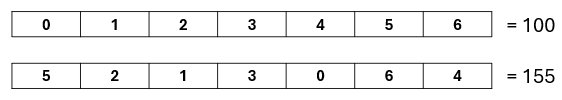
\includegraphics[width=0.8\textwidth]{
        papers/variationsprinzip_algorithmen/images/teil3/03_genetic_string_cities_results.png
        }
	\caption{Beispiel eines genetischen Strings mit Ergebnissen}
	\label{fig:cities_genetic_string_results}
\end{figure}


%
% teil3.tex -- Beispiel-File für Teil 3
%
% (c) 2020 Prof Dr Andreas Müller, Hochschule Rapperswil
%
% !TEX root = ../../buch.tex
% !TEX encoding = UTF-8
%
\subsection{Selektion
    \label{genetic_algorithm:selection}}
    \rhead{Selektion}
In diesem Schritt werden Elternpaare ausgesucht, die später 
neue Nachkommen erzeugen. Die Selektion erfolgt so, dass in der 
Regel nur die Fittesten neue Kinder erzeugen.

Die Idee dahinter ist, dass es verschiedene Individuen gibt, 
die unterschiedlich fit sind. Die fitteren Individuen paaren 
sich eher, während die schwächeren seltener Nachwuchs erzeugen. 
So ähnlich wie in der Natur. Die Paare werden im System zufällig 
gewählt, aber die Wahrscheinlichkeit, dass die fitteren 
Individuen Nachkommen zeugen, ist höher.

\begin{figure} [h]
    \centering
    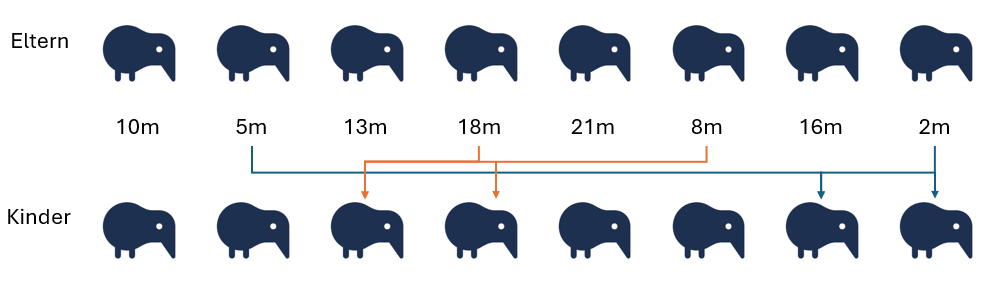
\includegraphics[width=0.8\textwidth]{
        papers/variationsprinzip_algorithmen/images/teil3/04_offspring_probability.png
    }
    \caption{Eltern die Ausgewählt werden für Nachkommen}
    \label{fig:selection_of_parents}
\end{figure}

Auf dem Bild \ref{fig:selection_of_parents} sind eltern mit unterschiedlichem
Weg länge. Dabei ist die Wahrscheinlichkeiten das sich die Blaue Linie ereignet 
viel grösser als die Rote Linie. Diese ist aber trotzdem möglich.
\\
Für die Selektion gibt es verschiedene Möglichkeiten.
\\
1. **Roulette-Rad-Selektion:** 
- Individuen werden zufällig und proportional zu ihrer 
Fitness ausgewählt. Die Wahrscheinlichkeit wird anhand ihrer 
Fitness definiert. Kürzere Strecken haben eine höhere Chance, 
ausgewählt zu werden. Die Wahrscheinlichkeit wird mit einer 
entsprechenden Formel berechnet.

\begin{equation}
    \label{eq:probability_fittest}
    P_i = \frac{f_i}{\sum_{j=1}^{N} f_j}
\end{equation}

2. **Rangselektion:**
- Individuen werden nach ihrer Fitness sortiert und basierend 
auf ihrem Rang ausgewählt. Die Wahrscheinlichkeit wird anhand 
des Rangs definiert.

\begin{equation}
    \label{eq:probability_rating}
    P_i = \frac{r_i}{\sum_{j=1}^{N} r_j}
\end{equation}

3. **Turnierselektion:**
- Eine Gruppe von Individuen wird zufällig ausgewählt, und 
das fitteste Individuum dieser Gruppe wird als Elternteil gewählt.

Es gibt auch die Möglichkeit, ein eigenes Selektionssystem zu entwickeln, 
das ein Ausscheidungsverfahren beinhaltet, aus dem schließlich ein 
Elternpaar hervorgeht. Das System folgt einem logischen Ablauf, wobei 
die Wahrscheinlichkeit mathematisch berechnet wird.

%
% teil3.tex -- Beispiel-File für Teil 3
%
% (c) 2020 Prof Dr Andreas Müller, Hochschule Rapperswil
%
% !TEX root = ../../buch.tex
% !TEX encoding = UTF-8
%
\subsection{Mutation
\label{genetic_algorithm:mutation}}
Der Startpunkt des genetischen Algorithmus ist die Initialisierung.
Dabei wird eine zufällige Population von möglichen Lösungen erstellt.
Diese wird als ein genetischer String dargestellt.

\begin{figure} [h]
	\centering
	
\includegraphics[width=0.8\textwidth]{
        papers/variationsprinzip_algorithmen/images/teil2/01_genetic_string.png
        }
	\caption{Beispiel von möglichen Genetic String}
	\label{fig:possible_genetic_string}
\end{figure}

Dabei wird in jeder Position das Gen aktiviert mit 1 oder deaktiviert mit 0.
Problematik für Stätte funktioniert dies nicht, da wir eine Stadt nicht
einfach aus oder anschalten können. Beim Gen wie oben ändert sich die funktioniert
an der Position nicht. Beispiel Feld 2 ist veranwortlich, dass die Farbe Grün
dargestellt wird. Bei den Städten ändert sich aber die Reihenfolge, da wird 
nicht einfach Ein oder ausgeschaltet. Zur einfachheit wird in den Stellen 
die Nummer der Stadt genommen.

\begin{figure} [h]
	\centering
	\includegraphics[width=0.8\textwidth]{
        papers/variationsprinzip_algorithmen/images/teil2/02_genetic_string_cities.png
        }
	\caption{Beispiel von Stätten in einem Genetic String dargestellt}
	\label{fig:cities_genetic_string}
\end{figure}


in Geld 2 wird immer die Farbe Grün angezeigt,  Ausserdem ändern nicht die Reihenfolge
der der Stätte, wodurch bei änderungen nicht nur die Position 
Bei den Stätten ist dies nicht einfach so umzusetzen da Bei einem Rucksack, welches einzelne Gegenstände hat 



%
% teil3.tex -- Beispiel-File für Teil 3
%
% (c) 2020 Prof Dr Andreas Müller, Hochschule Rapperswil
%
% !TEX root = ../../buch.tex
% !TEX encoding = UTF-8
%
\subsection{Mutation
\label{genetic_algorithm:mutation}}
Dieser Schritt sorgt dafür, dass zufällige Änderungen in 
den Genen stattfinden. Dadurch entstehen neue Gene, was den 
gesamten Lösungsraum vergrößert. Dies soll verhindern, 
dass nur noch gleiche Genmuster entstehen und ermöglicht 
die Erzeugung neuer Varianten. Ein guter Vergleich zum 
maschinellen Lernen ist der Versuch, aus einem lokalen 
Extrempunkt herauszukommen und nicht stecken zu bleiben.
Die Mutation findet auch nicht bei jedem Kind statt. Wie 
in der Natur können sie perzufall ausgelösst werden.
\\
Würde der genetische String nur aus 0 und 1 bestehen, 
würden zufällig Stellen ein- und ausgeschaltet. Dies 
ist mit den Städten jedoch nicht möglich, daher werden 
Teile miteinander vertauscht.

\begin{figure} [h]
	\centering
	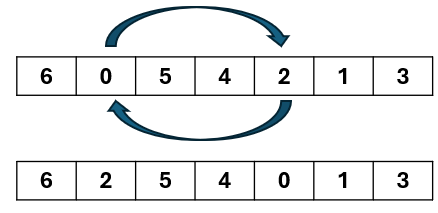
\includegraphics[width=0.8\textwidth]{
        papers/variationsprinzip_algorithmen/images/teil3/09_genetic_string_cities_mutation.png
        }
	\caption{Beispiel einer Mutation mit Städten}
	\label{fig:mutation_genetic_string}
\end{figure}

Dieser Teil besitzt keine mathematische Formel. Es geht einfach 
um die Logik, zwei zufällige Stellen zu nehmen und diese zu 
tauschen, um eine neue Variation von Lösungen zu erstellen, die 
bei der Kreuzung nicht entstanden wäre.

%
% teil3.tex -- Beispiel-File für Teil 3
%
% (c) 2020 Prof Dr Andreas Müller, Hochschule Rapperswil
%
% !TEX root = ../../buch.tex
% !TEX encoding = UTF-8
%
\subsection{Ersetzen
\label{genetic_algorithm:replacement}}
Der Ersetz schritt macht was er aussagt. Meistens wird die ganze 
Population durch die neue Ersetzt. Je nach Strategie macht es Sinn, dass 
die besten Population behalten werden. Wichtig ist das man die gesammt 
grösse der Generation nicht vergrössert, also von den neuen nur die besten 
halten bis der Satz voll ist.

%
% teil3.tex -- Beispiel-File für Teil 3
%
% (c) 2020 Prof Dr Andreas Müller, Hochschule Rapperswil
%
% !TEX root = ../../buch.tex
% !TEX encoding = UTF-8
%
\subsection{Abbruchkriteriums
\label{genetic_algorithm:termination}}
Was auch in Maschine Learning ein wichtiges Thema ist, ab welchem 
Zustand sollen die Berechnungen beendet werden. Beim generischen 
Algorithmus wird in der Regel eine Anzahl an Generationen definiert.
Möglich wäre auch, dass man ab einer gewissen Fittness Wert, die Lösung 
als genügend empfinden.



